\chapter{Planejamento} \label{cap:planejamento}

Afim de consolidar o planejamento do projeto de MPS deste trabalho foi estabelecido um Plano de Projeto que pode ser visto no
Apêndice \ref{plano_de_projeto}. Neste plano consta o planejamento de recursos humanos e o planejamento do tempo materializado
pelo cronograma. Para este projeto não foram considerados os custos envolvidos. 


\section{Embasamento da abordagem}

Para guiar a definição das ações de melhoria, alinhado com os objetivos de melhoria,
foram considerados os processos de Garantia de Qualidade de Software, de Gestão de Configuração,
de Gestão de Medição e Teste de Qualificação de Software da norma ISO/IEC 12207/2008 \cite{12207}, porque o propósito de ambos está 
de acordo com os objetivos de melhoria do projeto, podendo contribuir com atividades para o processo de melhoria.

De acordo com a norma ISO/IEC 12207/2008 \cite{12207}, os processos podem ser resumidos em seus respectivos propósitos e resultados:\\

\noindent
\textbf{Processo de Garantia de Qualidade de Software}
\begin{itemize}
    \item \textbf{Propósito}: \emph{Assegurar que os produtos de trabalho e processos estejam de acordo com os planos e provisões predefinidos.}
    \item \textbf{Resultados}:
        \subitem - Uma estratégia para conduzir a garantia de qualidade é desenvolvida;
	\subitem - Evidência da qualidade do software é produzida e mantida;
	\subitem - Problemas e não-conformidades com os requisitos são identificados e documentados;
	\subitem - A aderência dos produtos, processos e atividades aos padrões aplicáveis, procedimentos e requisitos é verificada.
\end{itemize}


\noindent
\textbf{Processo de Gestão de Configuração}
\begin{itemize}
    \item \textbf{Propósito}: \emph{Estabelecer e manter a integridade de todos os produtos identificados do projeto ou processo
	   e disponibilizá-los às partes interessadas.}
    \item \textbf{Resultados}:
        \subitem - Uma estratégia de gestão de configuração é definida;
	\subitem - Itens de configuração são definidos;
	\subitem - Baselines são estabelecidas;
	\subitem - Mudanças nos itens de configuração são gerenciadas e controladas;
	\subitem - A configuração de itens entregues é controlada;
	\subitem - O estado dos itens de configuração é disponibilizado ao longo do ciclo de vida.
\end{itemize}


\noindent
\textbf{Processo de Gestão de Medição}
\begin{itemize}
    \item \textbf{Propósito}: \emph{Coletar, analisar e comunicar dados relacionados aos produtos desenvolvidos e 
	  os processos implementados na organização, para dar suporte ao gerenciamento efetivo e demonstrar a qualidade dos produtos.}
    \item \textbf{Resultados}:
        \subitem - As necessidades de informação são identificadas;
	\subitem - Um conjunto apropriado de métricas, dirigido pelas necessidades de informação são identificados e/ou desenvolvidos;
	\subitem - Atividades de medição são identificas e planejadas;
	\subitem - Os dados necessários são coletados, armazenados, analisados e os resultados interpretados;
	\subitem - Produtos de informação são utilizados para suportar decisões e prover uma base objetiva para a comunicação;
	\subitem - O Processo de Medição e as métricas são avaliados;
	\subitem - Melhorias são comunicadas ao responsável pelo Processo de Medição.
\end{itemize}

\noindent
\textbf{Processo de Teste de Qualificação de Software}
\begin{itemize}
    \item \textbf{Propósito}: \emph{Confirmar que o produto integrado de software está de acordo com os requisitos definidos.}
    \item \textbf{Resultados}:
        \subitem - Critérios de aceitação para o produto de software são desenvolvidos para demonstrar a conformidade com os requisitos;
        \subitem - O software integrado é verificado utilizando os critérios definidos;
        \subitem - Os resultados dos testes são armazenados;
        \subitem - Uma estratégia de regressão é desenvolvida para retestar o software quando há mudanças.
\end{itemize}


A partir dos propósitos, resultados e atividades de cada processo da norma ISO/IEC 12207/2008 e no CMMI-DEV, foram levantadas as
ações de melhoria para alcançar os objetivos de melhoria propostos, que estão descritas na próxima seção. Vale ressaltar, que apenas os propósitos e
práticas considerados relevantes doram utilizados.

Além dos processos da norma ISO/IEC 12207/2008, alguns princípios e práticas ágeis do \textit{eXtreme Programming} (XP) \cite{xp} 
foram levados em conta para embasar a definição das ações de melhoria. São eles:

\begin{itemize}
 \item Rápido \textit{Feedback};
 \item Manter a simplicidade;
 \item Mudanças incrementais;
 \item Trabalho de qualidade;
 \item Testes;
 \item Refatoração;
 \item Integração contínua;
 \item Releases curtas.
\end{itemize}

O modelo de maturidade CMMI-DEV também foi utilizado como embasamento das ações de melhoria e foram escolhidos duas áreas de
processos relacionadas com os objetivos de melhoria: Gestão de Configuração (CM) e Integração de Produto (PI).
Os objetivos dessas áreas de processo podem ser sumarizadas nos seguintes itens:


\noindent
\textbf{Gestão de Configuração (CM)}
\begin{itemize}
    \item \textbf{Propósito}: \emph{Fornecer subsídios para estabelecer e manter a integridade dos produtos de
      trabalho, utilizando identificação de configuração, controle de configuração, balanço das atividades de configuração e auditorias de
      configuração \cite{cmmi}}
    \item \textbf{Práticas}:
        \subitem \textit{SG 1 Estabelecer Baselines}
	  \subsubitem SP 1.1 Identificar Itens de Configuração 
	  \subsubitem SP 1.2 Estabelecer um Sistema de Gestão de Configuração 
	  \subsubitem SP 1.3 Criar ou Liberar Baselines 
	\subitem \textit{SG 2 Acompanhar e Controlar Mudanças}
	  \subsubitem SP 2.1 Acompanhar Solicitações de Mudança 
	  \subsubitem SP 2.2 Controlar Itens de Configuração 
	 \subitem \textit{SG 3 Estabelecer Integridade }
	  \subsubitem SP 3.1 Estabelecer Registros de Gestão de Configuração
	  \subsubitem SP 3.2 Executar Auditorias de Configuração
\end{itemize}
		

\noindent
\textbf{Integração de Produto (PI)}
\begin{itemize}
    \item \textbf{Propósito}: \emph{Fornecer
subsídios para montar o produto a partir de componentes de produto,
assegurar que o produto integrado execute as funções de forma
apropriada e entregar o produto. \cite{cmmi}}
    \item \textbf{Práticas}:
		\subitem \textit{SG 1 Preparar-se para Integração de Produto}

			\subsubitem SP 1.1 Determinar Sequência de Integração
			\subsubitem SP 1.2 Estabelecer Ambiente de Integração do Produto
			\subsubitem SP 1.3 Estabelecer Procedimentos e Critérios para Integração do Produto
		\subitem \textit{SG 2 Assegurar Compatibilidade das Interfaces}
			\subsubitem SP 2.1 Revisar Descrições de Interfaces para Assegurar Completude
			\subsubitem SP 2.2 Gerenciar Interfaces
			\subsubitem SP 3.1 Confirmar se os Componentes do Produto estão Prontos para serem Integrados
		\subitem \textit{SG 3 Montar Componentes do Produto e Entregar Produto}
			\subsubitem SP 3.2 Montar Componentes do Produto
			\subsubitem SP 3.3 Avaliar Componentes de Produto Montados
			\subsubitem SP 3.4 Empacotar e Entregar Produto ou Componente de Produto
\end{itemize}


\vfill
\pagebreak
\section{Ações de melhoria}

Com os objetivos de melhoria definidos na fase de Iniciação foram estabelecidas ações para alcançá-los. Estas ações estão 
descritas na Tabela \ref{tab:acoes}. Os objetivos de melhoria foram priorizados de acordo com as necessidades da organização
alinhadas com a experiência da equipe de desenvolvimento no contexto.

\begin{table}[!h]
\centering
\caption{Ações de melhoria}
\label{tab:acoes}
\begin{tabular}{|c|c|l|l|}
\hline
\multicolumn{1}{|l|}{Prioridade} & \multicolumn{1}{l|}{Objetivo}                                                                                    & Ações                                                                                       & Produto                                                 \\ \hline
\multirow{4}{*}{1}               & \multirow{4}{*}{\begin{tabular}[c]{@{}c@{}}Formalizar o processo de \\ desenvolvimento de software\end{tabular}} & \begin{tabular}[c]{@{}l@{}}Implantar boas práticas de\\  métodos ágeis\end{tabular}         & \multicolumn{1}{c|}{\multirow{4}{*}{Processo modelado}} \\ \cline{3-3}
                                 &                                                                                                                  & \begin{tabular}[c]{@{}l@{}}Padronizar a execução das \\ atividades do processo\end{tabular} & \multicolumn{1}{c|}{}                                   \\ \cline{3-3}
                                 &                                                                                                                  & Modelar o processo                                                                          & \multicolumn{1}{c|}{}                                   \\ \cline{3-3}
                                 &                                                                                                                  & Validar o processo                                                                          & \multicolumn{1}{c|}{}                                   \\ \hline
\multirow{3}{*}{2}               & \multirow{3}{*}{\begin{tabular}[c]{@{}c@{}}Otimizar a atividade de \\ implantação\end{tabular}}                  & \begin{tabular}[c]{@{}l@{}}Definir atividades rigorosas \\ de implantação\end{tabular}      &                                                         \\ \cline{3-4} 
                                 &                                                                                                                  & \begin{tabular}[c]{@{}l@{}}Selecionar ferramenta de\\  integração contínua\end{tabular}     &                                                         \\ \cline{3-4} 
                                 &                                                                                                                  & Implantar integração contínua                                                               & Script                                                  \\ \hline
\multirow{2}{*}{3}               & \multirow{2}{*}{\begin{tabular}[c]{@{}c@{}}Estabelecer métricas \\ para o processo\end{tabular}}                 & Definir medições relevantes                                                                 &                                                         \\ \cline{3-4} 
                                 &                                                                                                                  & Definir plano de medição                                                                    & Plano de Medição                                        \\ \hline
\end{tabular}
\end{table}

Para o objetivo de melhoria "\emph{Formalizar o processo de desenvolvimento de software}", no processo a ser modelado as
seguintes atividades devem ser incluídas, baseando-se nas atividades dos processos de Garantia de Qualidade de Software,
de Gestão de Configuração e de Teste de Qualificação de Software da norma ISO/IEC 12207/2008 \cite{12207}. Algumas atividades
foram relacionadas com as práticas selecionadas do CMMI-DEV. 
 
\begin{itemize}
  \item Definir um subprocesso de garantia de qualidade;
    \subitem - Definir atividades para Garantia do Produto;
    \subitem - Definir atividades para Garantia do Processo;
    \subitem - Adicionar atividades de Verificação e Validação para a garantia da qualidade.
  \item Definir e padronizar a estratégia de gerência de configuração;
    \subitem - Definir estratégia para o controle de mudanças;
      \subsubitem CMMI: SP 2.1 Acompanhar Solicitações de Mudança e SP 2.2 Controlar Itens de Configuração 
  \item Estabelecer e manter suíte de testes;
    \subitem - Desenvolver critérios de aceitação para o software integrado, de acordo com os requisitos;
    \subitem - Montar suíte de testes;
    \subitem - Definir estratégia para testes de regressão;
    \subitem - Atualizar suíte de testes e documentação associada.
    \subitem - Documentar resultados dos testes;
\end{itemize}

O objetivo de melhoria "\emph{Otimizar a atividade de implantação}" consiste em facilitar a atividade de implantação,
para que o impacto da burocracia no acesso ao ambiente de produção seja mínimo no desenvolvimento do sistema.
Para atingir este objetivo, é proposta a adição da técnica de integração contínua ao processo para automatizar a
implantação e atualização do código. Esta proposta está alinhada com os princípios e práticas ágeis Rápido \textit{feedback},
Testes e Integração Contínua, propostos por \citeonline{xp} na metodologia XP. Além disso, as práticas do CMMI 
\textit{SP 1.2 Estabelecer Ambiente de Integração do Produto} e 
\textit{SP 1.3 Estabelecer Procedimentos e Critérios} para Integração do Produto da área de processo Integração 
do Produto corroboram com a criação da integração contínua.

O objetivo de melhoria "\emph{Estabelecer métricas para o processo}" seria basicamente um subprocesso 
do processo que será obtido com o objetivo "\emph{Formalizar o processo de desenvolvimento de software}", 
mas a sua importância para o contexto é tamanha que este foi destacado como um objetivo de melhoria por si só,
pois para que a melhoria possa ser visualizada é preciso métricas para acompanhar a evolução do processo.
Para este objetivo de melhoria, as seguintes atividades devem ser incluídas ao processo de medição,
baseado no processo de Gestão de Medição da norma ISO/IEC 12207/2008 \cite{12207}:

\begin{itemize}
 \item Identificar e priorizar as necessidades de informação;
 \item Selecionar e documentar as métricas a serem coletadas, que satisfaçam as necessidades de informação;
 \item Definir procedimentos de medição;
 \item Executar o processo de medição, seguindo os procedimentos;
    \subitem - Coletar, armazenar e verificar dados;
    \subitem - Analisar os dados e desenvolver produtos de informação;
    \subitem - Comunicar resultados;
 \item Avaliar produtos de informação, identificar e comunicar possíveis melhorias;
\end{itemize}

Para a definição das métricas o método GQM (Basili et al, 1994 apud \cite{solingen99}) se mostra adequado, 
pois apresenta um processo de medição bem estruturado, detalhado, dividido em diferentes níveis de abstração
e orientado a objetivos, também estando em conforme com as especificações do processo de Gestão de Medição
da norma ISO/IEC 12207/2008.

\section{Avaliação da melhoria}

A avaliação da melhoria seguirá o processo ilustrado na Figura \ref{fig:processo_avaliacao}.

\begin{figure}[!ht]
\centering
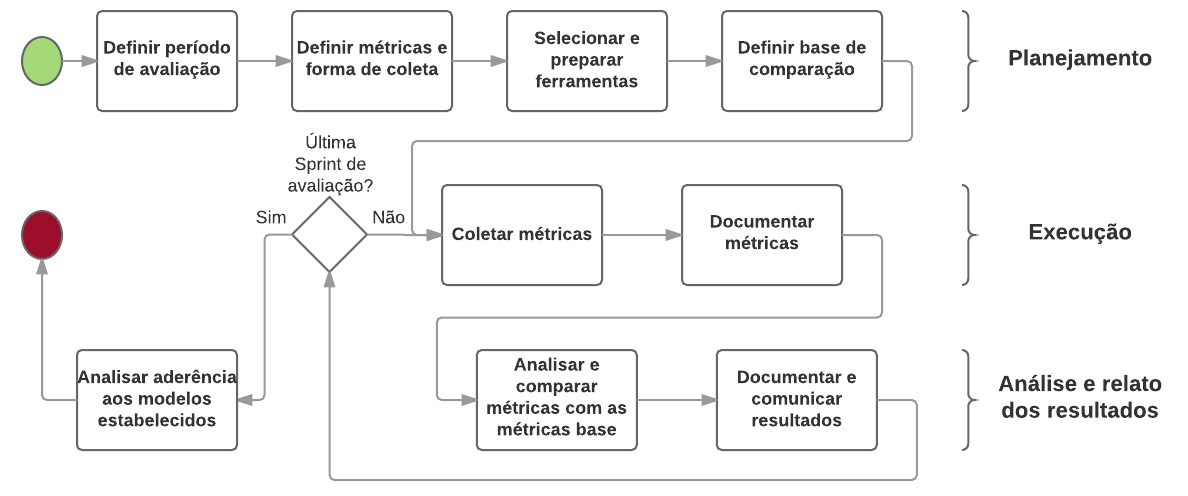
\includegraphics[scale=0.4]{figuras/processo_avaliacao.png}
\caption{Processo de avaliação das melhorias}
\label{fig:processo_avaliacao}
\end{figure}

O Planejamento da Avaliação consiste em atividades introdutórias à avaliação como definição do período de avaliação,
definição de métricas, ferramentas e formas de coleta e a definição da base de comparação. A base de comparação consiste
em valores de referência das métricas definidas para averiguar se houve melhorias ou não ao longo da execução do processo de melhoria.

A Execução e Análise e Relato dos Resultados da Avaliação consiste em atividades para coleta e interpretação das métricas,
que são realizadas em ciclos durante o período de avaliação definido anteriormente. Por fim, ao final dos ciclos de execução 
e análise o novo processo e os produtos de trabalho gerados são confrontados frente aos modelos ISO/IEC 12207/2008 e CMMI, e às práticas ágeis 
para verificar sua aderência aos mesmos.

\subsection{Planejamento da avaliação}
    
    Para avaliar o resultado do processo de melhoria será executada uma avaliação de confronto com os elementos selecionados
    da 12207, do CMMI-DEV e das práticas ágeis. A fim de comparar o processo melhorado com o processo atual a mesma avaliação 
    de confronto foi realizada no processo atual e pode ser vista no Apêndice \ref{ap:avaliacao}. As mesmas tabelas serão 
    utilizadas para avaliação do processo melhorado.
    
    Além disso, serão coletadas as seguintes métricas para avaliar o resultado do processo de melhoria:
    
    \begin{itemize}
      \item \textbf{Número de desvios ao processo};
	\subitem Esta métrica permitirá acompanhar a aderência da equipe ao novo processo, informando a quantidade
		 de vezes em que atividades do processo definido não foram seguidas. Esta métrica será levantada durante
		 a Revisão da \textit{Sprint}, realizando uma verificação da atuação na \textit{Sprint}.
      \item \textbf{Número de defeitos por atualização de código};
	\subitem Esta métrica visa contabilizar a quantidade de defeitos percebidos pela equipe decorrentes de novos
		 incrementos de \textit{software} em ambiente de homologação. Esta métrica será coletada pela equipe 
		 durante a Revisão da \textit{Sprint}.
      \item \textbf{Número de defeitos decorrentes da implantação};
	\subitem Esta métrica visa contabilizar a quantidade de defeitos percebidos tanto pela equipe quanto por usuários 
		 decorrentes de atualizações de código no ambiente de produção.
      \item \textbf{Cobertura de código}.
	\subitem Esta métrica permitirá acompanhar a evolução dos testes no processo de desenvolvimento e será coletada por meio da
		 ferramenta PHPUnit \footnotemark. \footnotetext{https://phpunit.de/}
    \end{itemize}
    
    A avaliação das melhorias será comparada com valores base das métricas acima. Para determinar os valores base para comparação, 
    as métricas definidas acima serão coletadas em um período de duas \textit{sprints} e será realizada uma média dos valores.
    
    Como o desenvolvimento do SiGA segue o \textit{framework Scrum}, as ações implementadas serão avaliadas semanalmente,
    no fim de cada \textit{Sprint} durante 8 \textit{Sprints} (2 meses), a partir da coleta das métricas definidas acima e
    comparação com os valores base.
